\section{Uranerz}

\subsection{Gammaspektrum}

In diesem Versuchsteil wollen wir schauen, welche Elemente wir anhand des Gammaspektrums des Uranerzen in diesem nachweisen können. Dazu haben 
wir haben das Uranerz eine Stunde auf unserem Ge-Detektor gestellt, um auch die schwächeren Linien über das Rauschen zu heben.\\
In der daraus entstehenden Abbildung \ref{Uranerz} kann man deutlich die charakteristischen Linien herrauslesen und zuzuordnen\footnotemark.
\footnotetext{\url{https://de.wikipedia.org/wiki/Gammaspektroskopie}, Eingesehen am 15.09.2021}

\begin{figure}[h]
    \centering
    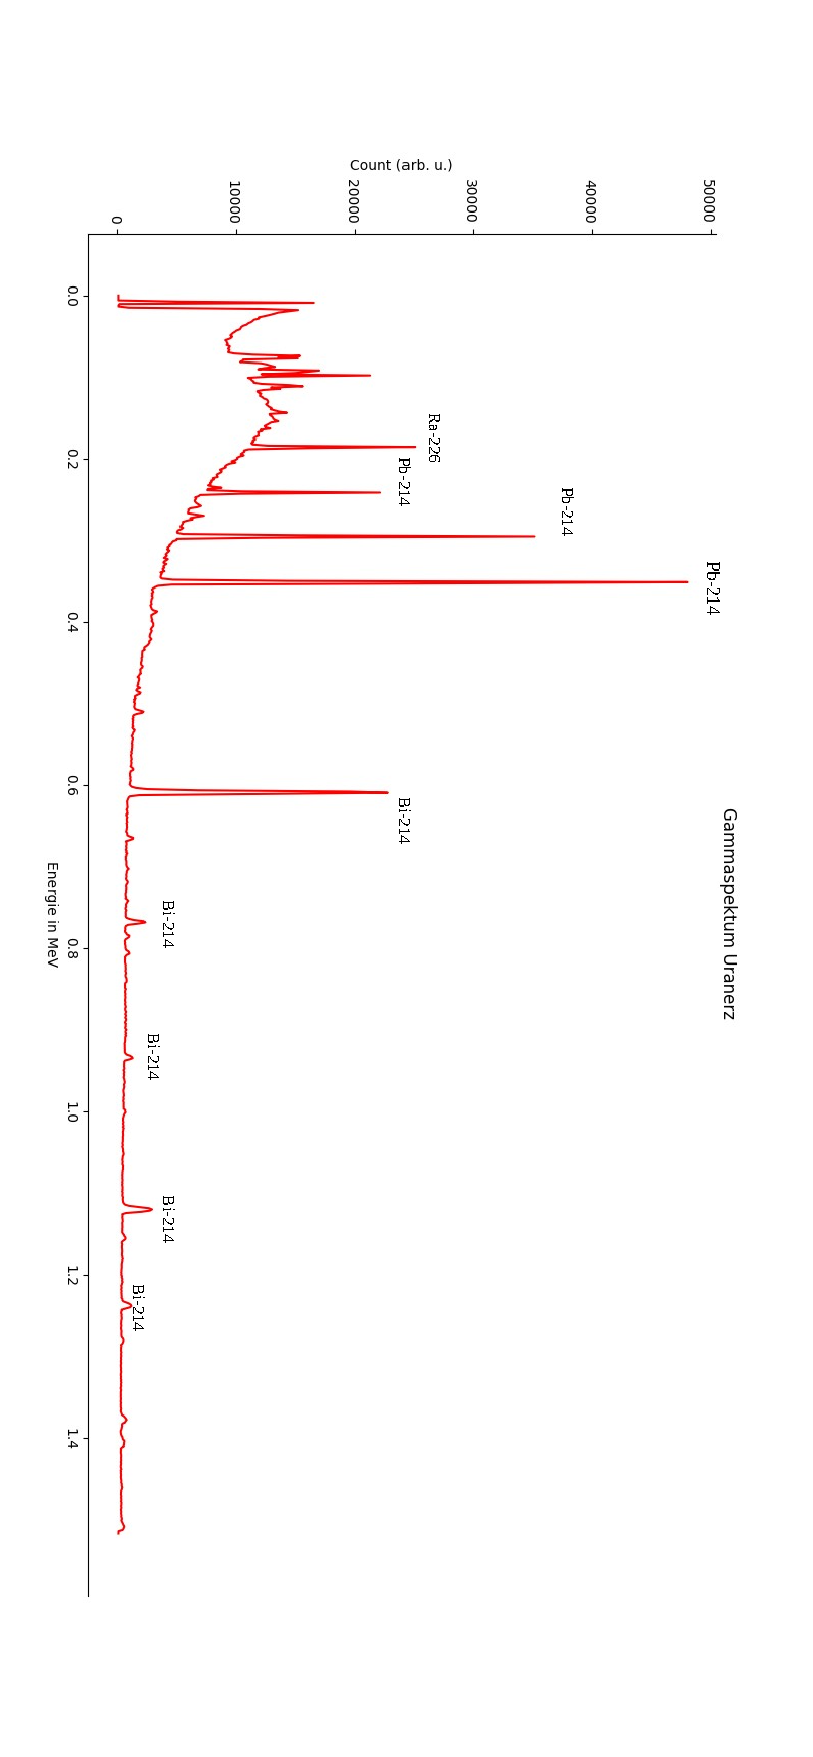
\includegraphics[width = 12cm]{Bilder/Auswertung/UranerzSpektrum.pdf}
    \caption{Spektrum des Uranerz}
    \label{Uranerz}
\end{figure}

\clearpage
\subsection{Massenabsorptionskoeffizient}

Nun wiederholen wir die Messung aus Kapitel \ref{section:Absorbtionskoeff} mit Blei. Dabei haben wir diesmal den Vorteil, dass wir aufgrunde der vielen 
Spektrallinien die Energieabhängigkeit des Massenabsorptionskoeffizient beobachten können. Dafür haben wir eine leere Messung, eine Messung mit 1,2,3,4 und 7 Bleiplatten mit 
jeweils einem Millimeter zu Verfügung. Die Absorptionskoeffizienten  werden exemplarisch an drei Linien berechnet. 